% Created 2022-07-01 Fri 15:24
% Intended LaTeX compiler: pdflatex
\documentclass[presentation,aspectratio=169]{beamer}
\usepackage[utf8]{inputenc}
\usepackage[T1]{fontenc}
\usepackage{graphicx}
\usepackage{grffile}
\usepackage{longtable}
\usepackage{wrapfig}
\usepackage{rotating}
\usepackage[normalem]{ulem}
\usepackage{amsmath}
\usepackage{textcomp}
\usepackage{amssymb}
\usepackage{capt-of}
\usepackage{hyperref}
\usepackage{khpreamble}
\usepackage{amssymb}
\usepackage{mathtools}
\usepgfplotslibrary{groupplots}
\DeclareMathOperator{\shift}{q}
\DeclareMathOperator{\diff}{p}
\usetheme{default}
\author{Kjartan Halvorsen}
\date{2022-07-01}
\title{Delay and phase shift}
\hypersetup{
 pdfauthor={Kjartan Halvorsen},
 pdftitle={Delay and phase shift},
 pdfkeywords={},
 pdfsubject={},
 pdfcreator={Emacs 26.3 (Org mode 9.4.6)}, 
 pdflang={English}}
\begin{document}

\maketitle

\section{Delay}
\label{sec:orgcb102a2}

\begin{frame}[label={sec:org03dec3b}]{Delay and phase lag}
\begin{center}
  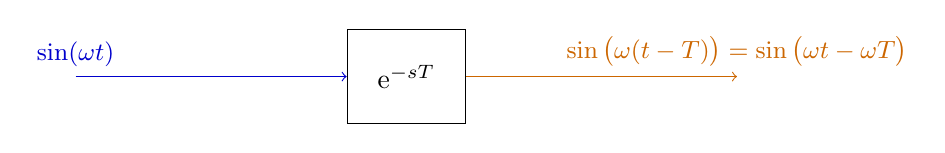
\begin{tikzpicture}[node distance=20mm, block/.style={rectangle, draw, minimum width=15mm, minimum height=12mm}]

    \node[coordinate] (input) {};
    \node[block, right of=input, node distance=42mm] (lti) {$\mathrm{e}^{-sT}$};
    \node[coordinate, right of=lti, node distance=42mm] (output) {};

    \draw[->, blue!80!black] (input) -- node[above, at start] {\small $\sin(\omega t)$} (lti);
    \draw[->, orange!80!black] (lti) -- node[above, at end] {\small $\sin\big(\omega(t-T)\big) = \sin\big(\omega t - \omega T\big)$} (output);
  \end{tikzpicture}
\end{center}

\pause

\begin{center}
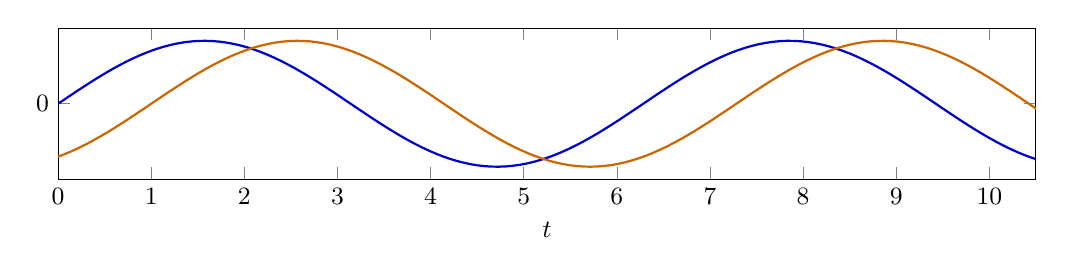
\begin{tikzpicture}
\small
\pgfmathsetmacro{\ww}{1}
\pgfmathsetmacro{\TT}{2*pi/\ww}
\begin{axis}[
width=14cm,
height=3.5cm,
xlabel={$t$},
xmin=0.,
xmax=10.5,
ytick = {0},
%xtick = {0, \TT},
%xticklabels={0, $2\pi$},
]
\addplot+[blue!80!black, thick,no marks, domain=0:30, samples=400,variable=t] { sin(deg(\ww*t)) };
\addplot+[orange!80!black, thick,no marks, domain=0:30, samples=400,variable=t] { sin(deg(\ww*(t-1))) };
\end{axis}
\end{tikzpicture}
\end{center}

\pause

\alert{Activity} Determine the frequency \(\omega\) of the sine waves, the delay \(T\) and the phase lag \(\omega T\).
\end{frame}
\end{document}